Words can be grouped together into equivalence classes to help reduce data sparsity and better generalize data. Word clusters can be seen as an intermediate representation of knowledge that is more descriptive than a flat list of terms and less expressive than a full ontology. As such, we consider word clusters to be \textbf{\textit{sub-ontological knowledge}} that can be easily incorporated into many NLP and MT applications without the overhead of considering the full graphical representation of an ontology.

Within machine translation word classes are used in word alignment \citep{brown-etal1993,och-ney2000}, factored machine translation \citep{koehn-hoang2007} and translation models \citep{koehn-hoang2007,wuebker-etal2013}, reordering \citep{cherry2013}, preordering \citep{stymne2012}, target-side inflection \citep{chahuneau-etal2013}, SAMT \citep{zollmann-vogel2011}, sparse word features \citep{haddow-etal2015}, and OSM \citep{durrani-etal2014}, among many others.

Word clusterings have also found utility in parsing \citep{koo-etal2008,candito-seddah2010,kong-etal2014}, semantic parsing \citep{zhao-etal2009}, chunking \citep{turian-etal2010}, NER \citep{miller-etal2004,liang2005,ratinov-roth2009,ritter-etal2011}, tweet tagging \citep{owoputi-etal2013,nooralahzadeh-etal2014}, structure transfer \citep{tackstrom-etal2012}, and discourse relation discovery \citep{rutherford-xue2014}.

Word clusters are useful in training neural and MaxEnt language models. Word clusters also speed up normalization in training neural network and MaxEnt language models, via class-based decomposition \citep{goodman2001a}. This reduces the normalization time from $\mathcal{O}(|V|)$ (the vocabulary size) to $\approx \mathcal{O}(\sqrt{|V|})$\,. Further improvements to $\mathcal{O}(\log(|V|))$ are found using hierarchical softmax \citep{morin-bengio2005,mnih-hinton2009}\,.\footnote{Part of the research presented in this chapter has been previously published in \cite{dehdari-etal2016}, \cite{dehdari-tan-vangenabith:2016:N16-1} and \cite{tan:2016:WAT2016}}

\section{Exchange-based Word Clustering}

Word clustering partitions a vocabulary $V$\!, grouping together words that function similarly. This helps generalize language and alleviate data sparsity. We discuss flat clustering in this section of the thesis. Flat, or strict partitioning clustering maps word types onto a smaller set of clusters.

The \textbf{exchange algorithm} \citep{kneser-ney1993} is an efficient technique that exhibits a general time complexity of 
$\mathcal{O}(|V| \times |C| \times I)$, where %
$|V|$ is the number of word types, %
$|C|$ is the number of classes, and $I$ is the number of training iterations, typically $<20$\,.
This omits the specific method of exchanging words, which adds further complexity.
Words are exchanged from one class to another until convergence or $I$\,.

One of the oldest and still most popular exchange algorithm implementations is {\tt mkcls} \citep{och1995}, which adds various metaheuristics to escape local optima. \cite{botros-etal2015}  introduce their implementation of three exchange-based algorithms \citep{martin-etal1998,mueller-schuetze2015}\footnote{use trigrams within the exchange algorithm.}. \cite{clark2003} adds an orthotactic bias.

The previous algorithms use an unlexicalized (two-sided) language model: % for the calculation of log-likelihood, the objective function:
$
	P(w_i|w_{i-1}) = P(w_i|c_i) \, P(c_i|c_{i-1})
$\,,
where the class $c_i$ of the predicted word $w_i$ is conditioned on the class $c_{i-1}$ of the previous word $w_{i-1}$\,.
\cite{goodman2001} altered this model so that $c_i$ is conditioned directly upon $w_{i-1}$\,, hence:
$
	P(w_i|w_{i-1}) = P(w_i|c_i) \, P(c_i|w_{i-1})
$\,.
This new model fractionates the history more, but it allows for a large speedup in hypothesizing an exchange since the history doesn't change.
The resulting partially lexicalized (one-sided) class model gives the accompanying \textbf{predictive exchange algorithm} \citep{goodman2001,uszkoreit-brants2008} a time complexity of
$\mathcal{O}((B + |V|) \times |C| \times I)$
where $B$ is the number of unique bigrams in the training set.

\cite{dehdari-tan-vangenabith:2016:N16-1} developed a \emph{bidirectional, interpolated, refining, and alternating} ({\tt BIRA}) predictive exchange algorithm. The goal of {\tt BIRA} is to produce better clusters by using multiple, changing models to escape local optima. This uses both forward and reversed bigram class models to improve cluster quality by evaluating log-likeli\-hood on two different models. Unlike using trigrams, bidirectional bigram models only linearly increase time and memory requirements, and in fact some data structures can be shared.
The two directions are interpolated to allow softer integration of these two models:

%\begin{equation}
%P(w_{ i }|w_{ i-1 },w_{ i+1 }) \triangleq P(w_{ i }|c_{ i }) \cdot (\lambda P(c_{ i }|w_{ i-1 }) +(1-\lambda )P(c_{ i }|w_{ i+1 }))
%\end{equation}

\begin{equation}
P(w_{ i }|w_{ i-1 },w_{ i+1 }) = P(w_{ i }|c_{ i }) \cdot (\lambda P(c_{ i }|w_{ i-1 }) +(1-\lambda )P(c_{ i }|w_{ i+1 }))
\end{equation}


The interpolation weight $\lambda$ for the forward direction alternates to \,$1-\lambda$\, every $a$ iterations ($i$): 

\begin{equation}
\lambda_i := \begin{cases}
	\ 1-\lambda_0 & \mbox{if \ \ } i \ \text{mod} \  a = 0 \\
	\ \lambda_0 & \mbox{otherwise}
\end{cases}
\end{equation}

The time complexity is $\mathcal{O}(2 \times (B + |V|) \times |C| \times I)$\,.
The original predictive exchange algorithm can be obtained by setting $\lambda=1$ and $a=0$\,.%
\footnote{The time complexity is $ \mathcal{O}((B + |V|) \times |C| \times I) $ if $\lambda=1$\,.}

\section{Experimental Setup}

We evaluated the word clusters from the {\tt BIRA} predictive exchange algorithm extrinsically in machine translation. As discussed in the previous section, word clusters are employed in a variety of ways within machine translation systems, the most common of which is in word alignment where {\tt mkcls} is widely used. As training sets get larger every year, {\tt mkcls} struggles to keep pace, and is a substantial time bottleneck in MT pipelines with large datasets. We compare time and BLEU scores of using {\tt mkcls} vs {\tt BIRA} in word alignment.

Similar to the experiments in Chapter 3 (Section 3.5), we used data from the Workshop on Machine Translation 2015 (WMT15) Russian-English dataset and the Workshop on Asian Translation 2014 (WAT14) Japanese-English dataset using the phrase-based machine translation configurations as described in Chapter 2 (Section 2.4). 

\section{Results}

\begin{table}[H]
\centering
\begin{tabular}{r|ll|ll}
$|C|$ & \bf EN-RU  & \bf RU-EN  & \bf EN-JA  & \bf JA-EN  \\ \hline

10         & 20.8$\rightarrow$20.9$^*$ & 26.2$\rightarrow$26.0         &  23.5$\rightarrow$23.4     &  16.9$\rightarrow$16.8 \\
50         & 21.0$\rightarrow$21.2$^*$ &  25.9$\rightarrow$25.7        &  24.0$\rightarrow$23.7$^*$ &  16.9$\rightarrow$16.9 \\
100        & 20.4$\rightarrow$21.1     &  25.9$\rightarrow$25.8        &  23.8$\rightarrow$23.5     &  16.9$\rightarrow$17.0 \\
200        & 21.0$\rightarrow$20.8     &  25.8$\rightarrow$25.9        &  23.8$\rightarrow$23.4     &  17.0$\rightarrow$16.8 \\
500        & 20.9$\rightarrow$20.9     &  25.8$\rightarrow$25.9$^*$    & 24.0$\rightarrow$23.8      & 16.8$\rightarrow$17.1$^*$ \\
1000       & 20.9$\rightarrow$21.1     &  25.9$\rightarrow$26.0$^{**}$ &  23.6$\rightarrow$23.5     &  16.9$\rightarrow$17.1 \\
\end{tabular}
\caption{BLEU scores \texttt{mkcls}$\rightarrow$\texttt{BIRA} and significance across cluster sizes (\,$|C|$\,)}
\label{table:mkcls2bira}
\end{table}

\begin{table}[H]
\centering
\begin{tabular}{r|lllll} % one-col
	%\#Clusters & & \multicolumn{1}{c}{EN-RU} & \multicolumn{1}{c|}{RU-EN} & \multicolumn{1}{c}{EN-JA} & \multicolumn{1}{c|}{JA-EN} \\ % two-col
	\bf \#Clusters & \hspace{0.3em} & \multicolumn{1}{c}{\bf EN-RU} & \multicolumn{1}{c}{\bf RU-EN} & \multicolumn{1}{c}{\bf EN-JA} & \multicolumn{1}{c}{\bf JA-EN} \\ % one-col
	\hline
	10         & &$ +0.1^*	$&$ -0.2		$&$ -0.14		$&$ -0.1	$\\
    50         & &$ +0.2^*	$&$ -0.2		$&$ -0.32 ^*	$&$ -0.04	$\\
    100        & &$ +0.7		$&$ -0.1		$&$ -0.27		$&$ +0.12	$\\
    200        & &$ -0.2		$&$ +0.1    	$&$ -0.35   	$&$ -0.15	$\\
	500        & &$ \,\,\,\,\,0	$&$ +0.1^*	 	$&$ -0.29   	$&$ +0.27^*	$\\
	1000       & &$ +0.2		$&$ +0.1^{**}	$&$ -0.07    	$&$ +0.13	$\\
\end{tabular}
\caption{BLEU score changes and significance across cluster sizes.}
\label{table:deltabira}
\end{table}

Table \ref{table:mkcls2bira} presents the absolute BLEU score changes and their statistical significance across cluster size (\,$|C|$\,).  Table \label{table:deltabira} summarizes the change in BLEU scores when replacing word clusters generated by \texttt{mkcls} with clusters from \texttt{BIRA}\footnote{Positive values indicate improvements made by replacing   \texttt{mkcls} with \texttt{BIRA}}. The BLEU score differences between using {\tt mkcls} and our {\tt BIRA} implementation are small but there are a few statistically significant changes\footnote{(*: $p$-value $<$ 0.05, **: $p$-value $<$ 0.01)}, using bootstrap resampling \cite{koehn2004significance}.

The maximum difference in BLEU score in any configuration is 0.7 absolute points (EN-RU, $|C|=100$, \texttt{BIRA} $=21.1$, {\tt mkcls} $= 20.4$, $p=0.32$). We ran the hypothesis tests twice per configuration, and there were no disagreements between each hypothesis testing. Nonetheless, \texttt{MERT} tuning is quite erratic, and some of the BLEU differences could be affected by noise in the tuning process in obtaining quality weight values.


\begin{figure}[!htb]
	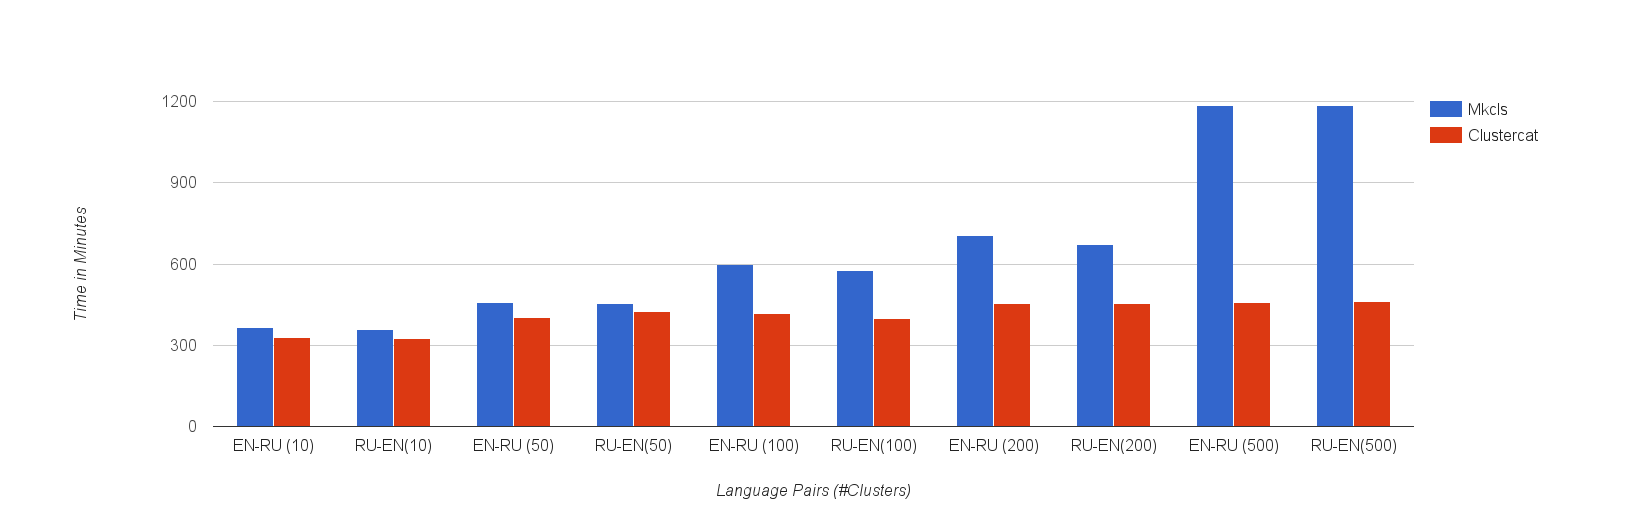
\includegraphics[width=\textwidth]{images/mt-training-times.png} 
	\caption{End-to-end translation model training times for English-Russian and Russian-English for various cluster sizes using \texttt{mkcls} and \texttt{BIRA}.}
	\label{fig-mt-training-times}
\end{figure}

Figure \ref{fig-mt-training-times} shows that \texttt{BIRA} enables MT experiments to explore high cluster sizes without the time-consuming overhead of \texttt{mkcls}. Using the {\tt BIRA} clustering algorithm reduces the translation model training time with 500 clusters from 20 hours using {\tt mkcls} (of which 60\% of the time is spent on clustering) to just 8 hours (of which 5\% is spent on clustering). It takes 8 hours to complete the full translation model training with 500 clusters, as compared to 20 hours using {\tt mkcls}. We bring the time for clustering from 60\% of the total training time to just 5\%\,.This reduces 5\% of the total training time for the {\tt BIRA} clusterer, compared to 60\% for {\tt mkcls}. Using our {\tt BIRA} implementation it takes 9 hours to complete the full translation model training with 1000 clusters, as compared to 30 hours using {\tt mkcls} -- 7\% of the total training time for the {\tt BIRA} clusterer, compared to 74\% for {\tt mkcls}.

\section{Summary}

In this Chapter, we incorporated sub-ontological structures (i.e. word clusters) into machine translation through improving the predictive exchange algorithm that address longstanding drawbacks of the original algorithm compared to other clustering algorithms and showed that word alignment models using the \texttt{BIRA} implementation fully match those using \texttt{mkcls} in BLEU scores, with time savings found by using our improvements.\footnote{The software is freely available at \url{https://github.com/jonsafari/clustercat}.}


